\section{Option pricing}
\subsection{The fundamental theorem of asset pricing}

\subsection{The Black-Scholes model}
Consider a given probability space $(\Omega, (\mathcal{F})_t,\mathbb{P})$ 
supporting a Brownian motion~$(W_t)_{t\geq 0}$.
In the Black-Scholes model, the stock price process~$(S_t)_{t\geq 0}$ is the unique strong solution to
the following stochastic differential equation:
\begin{equation}\label{eq:BS}
\frac{\D S_t}{S_t} = r \D t + \sigma \D W_t,
\qquad S_0>0,
\end{equation}
where $r\geq 0$ denotes the instantaneous risk-free interest rate and $\sigma>0$ the instantaneous volatility.

\subsubsection{No interest rates}
\subsubsection{Including interest rates}
A European call price $C_t(S_0,K,\sigma)$ with maturity $t>0$ and strike $K>0$ 
pays at maturity $(S_t-K)_+=\max(S_t-K,0)$. 
When the stock price follows the Black-Scholes SDE~\eqref{eq:BS}, 
Black and Scholes~\cite{blackholes} proved that its price at inception is worth
$$
C_t(S_0,K,\sigma) = S_0\mathcal{N}(d_+) - K\E^{-rt}\mathcal{N}(d_-),
$$
where
$$
d_{\pm} := \frac{\log\left(S_0 \E^{rt}/K\right)}{\sigma\sqrt{t}} \pm \frac{\sigma\sqrt{t}}{2},
$$
and where~$\mathcal{N}$ denotes the cumulative distribution function of the Gaussian random variable.

Here is an example of how to insert a picture:

\begin{figure}[!ht]
\centering
\subfigure{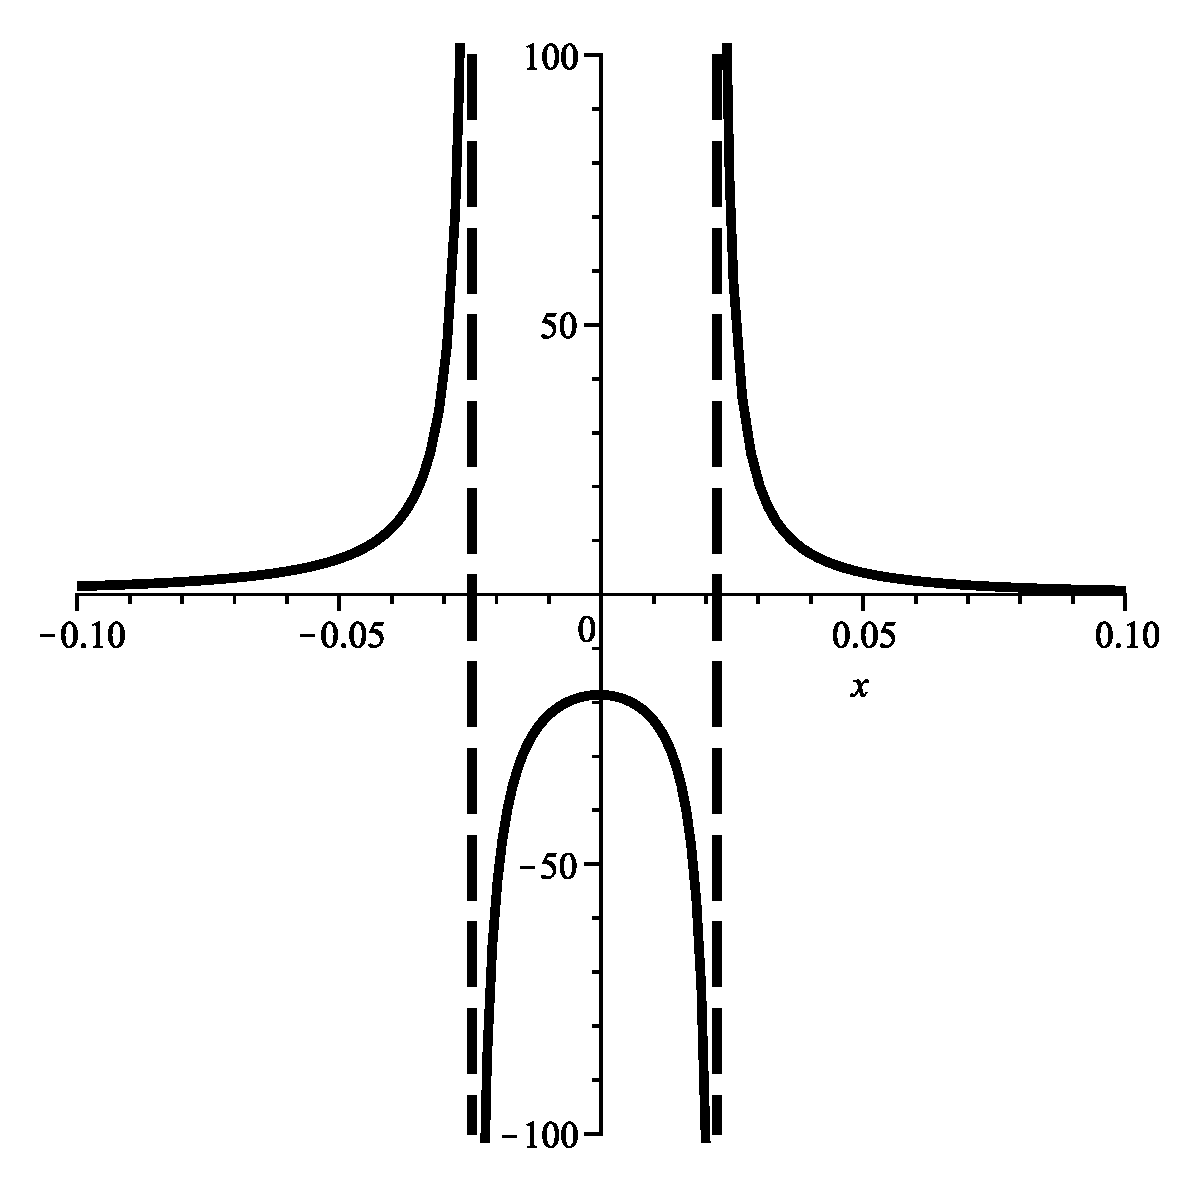
\includegraphics[scale=0.2]{figures/Picture.eps}}
\caption{This is the caption for the figure.}
\label{fig:Pict}
\end{figure}

or two side-by-side pictures:

\begin{figure}[!ht]
\centering
\subfigure{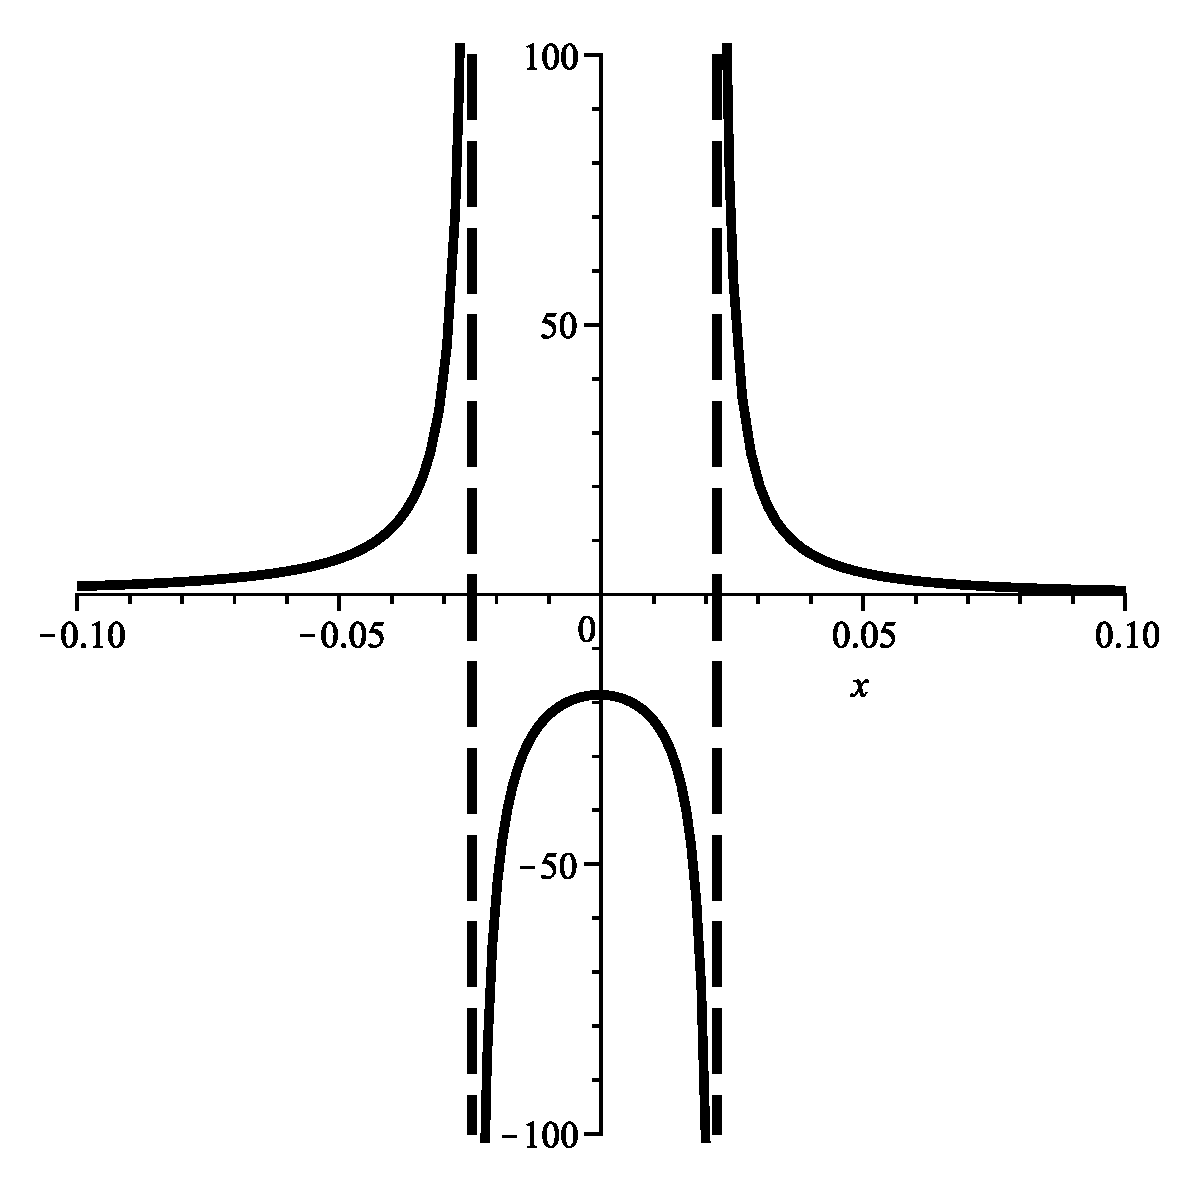
\includegraphics[scale=0.3]{figures/Picture.eps}}
\hspace{15pt}
\subfigure{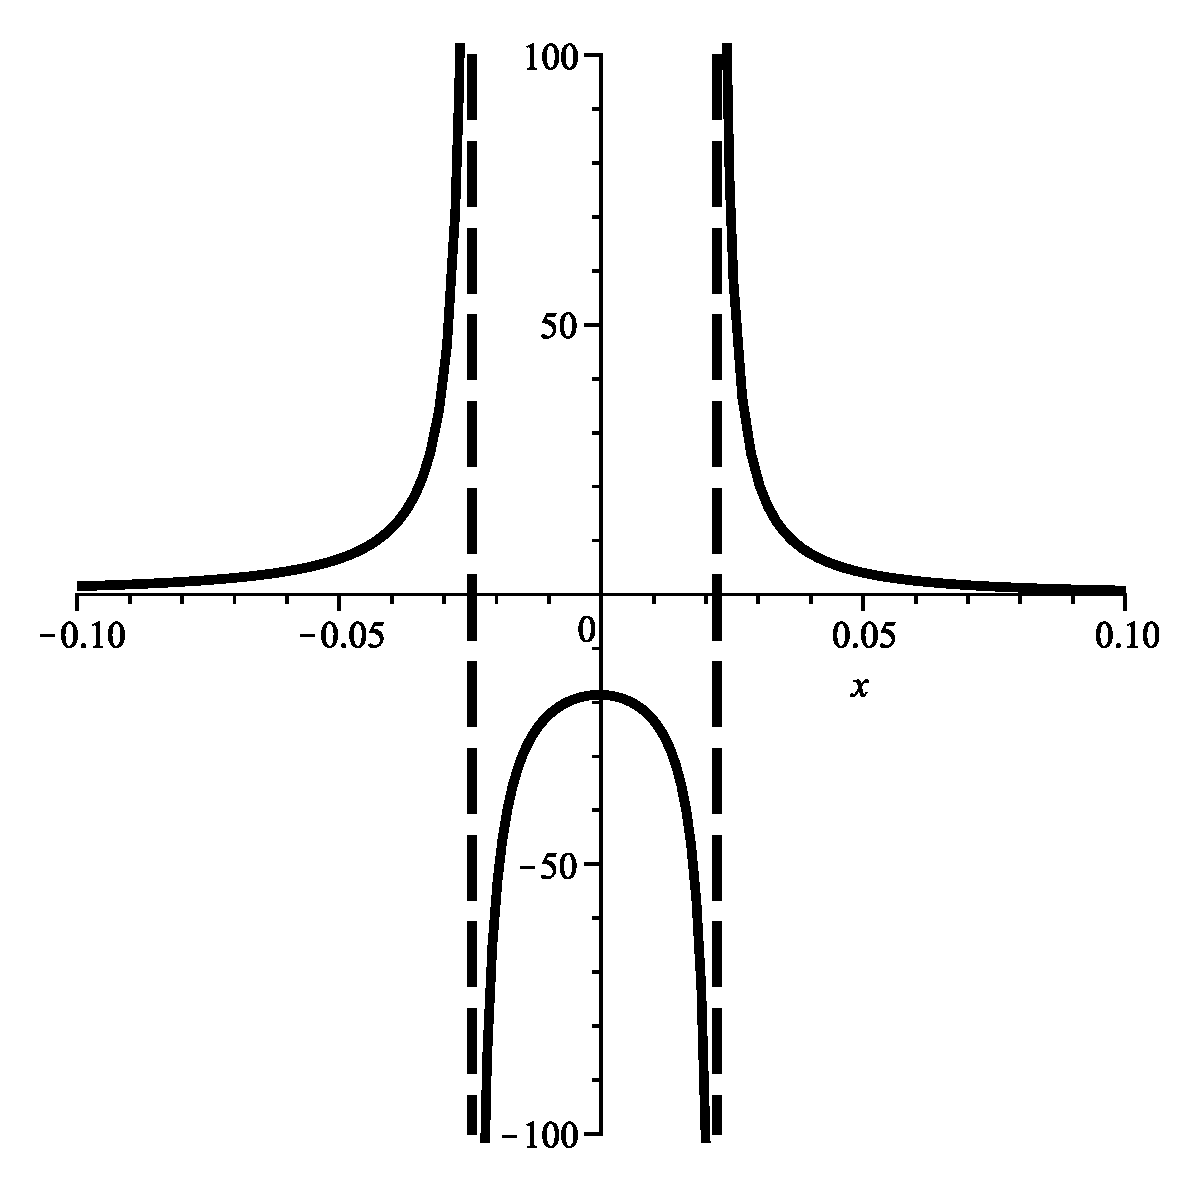
\includegraphics[scale=0.3]{figures/Picture.eps}}

\caption{Another caption}
\label{fig:Pict2}
\end{figure}

\subsection{The Heston model}
In the Heston model, the stock price is the unique strong solution to the following stochastic differential equation:
\begin{equation}\label{eq:Heston}
\begin{array}{rll}
\D S_t & = S_t \sqrt{V_t} \D W_t, & S_0 = s>0,\\
\D V_t & = \kappa(\theta-V_t)\D t + \xi\sqrt{V_t}\D Z_t, & V_0 = v_0>0,\\
\D \langle W, Z\rangle_t & = \rho \D t,
\end{array}
\end{equation}
where $\kappa, \xi, \theta, v_0, s>0$ and the correlation parameter $\rho$ lies in $[-1,1]$.
